\documentclass{article}
\usepackage[utf8]{inputenc}
\usepackage{geometry} 
\geometry{a4paper}  
%\usepackage[parfill]{parskip} 
\usepackage{graphicx}	
\usepackage{amsmath}
\usepackage{fullpage}
\usepackage{setspace} 
\usepackage{lineno}
\usepackage[none]{hyphenat}
\usepackage{listings}

\usepackage[round]{natbib}	

\title{Reproducible, flexible and high throughput data extraction from primary literature: The metaDigitise R package}
\author{Joel L. Pick, Shinichi Nakagawa \& Daniel W.A. Noble}
% \date{}

\begin{document}
\doublespacing
%\raggedright

\maketitle
Prepared for: Journal of Statistical Software

\section*{Abstract}

Keywords: meta-analysis, comparative analysis, data extraction, R, reproducibility, figures, images, summary statistics

\clearpage
\section*{Introduction}

Meta-analysis is becoming increasingly common in many research fields. They make use of various summary statistics from studies to generate effect size estimates and their sampling error variance to understand whether particular experimental manipulations, or relationships between variables, show strong overall effects and attempt to explain variation among these effects (Nakagawa et al. 2017). Meta-analysis relies foremost on data extracted from primary literature – more specifically statistics that have been reported in the text or tables of research papers. However, necessary summary statistics are often presented in figures, and so, these need to be manually extracted using digitising programs to be used in the final analysis. Although there are several existing tools to perform tasks like this, these tools are not made for this specific purpose (i.e. a meta-analysis). Specifically, they do not differentiate between common plot types that are use to present data, meaning that they require a large amount of downstream data manipulation. For example, many stand alone programs only provide the raw data or values from plots. This means that these data need to be imported into other programs to calculate correlations (if scatter plots) or errors on means (from mean error plots) need to be back calculated by hand to convert them to a common type (e.g., standard errors to standard deviations). Digitising programs also do not easily allow for different grouping of points to be made, and frequently do not integrate metadata (such as variable names, group names and sample sizes) at the time of data extraction. Additionally, existing stand-alone software does not allow easy import into commonly used statistical software (such as R), or try to optimize the research pipelines to facilitate editing and reproducibility. These are major issues because extracting from figures can be an incredibly time-consuming process. Furthermore, meta-analyses can have a major impact on research fields, and should be expanded upon as more research comes to light. Having a tool that facilitates reproducibility in meta-analyses will increase transparency and go a long way to resolving the reproducibility crises we are seeing in many fields.

Here, we present an interactive R package, `metaDigitise`, which is designed for large scale data extraction from figures, specifically catering to the the needs of meta-analysts. To this end, we provide tools specific to data extraction from common plot types (mean and error plots, box plots, scatter plots and histograms, see Figure \ref{fig:plot_type}). `metaDigitise` operates within the R environment making data extraction, analysis and export more streamlined. It also provides users with options to conduct the necessary calculations on raw data immediately after extraction so that comparable summary statistics can be obtained quickly. Summaries will condense multiple figures into data frames or lists (depending on the type of figures) and these objects can easily be exported from R, or if using the raw data, analysed in any way the user desires. Conveniently, when needing to process many figures at different times `metaDigitise` will only import figures not already completed within a directory. This makes it easy to add new figures at anytime. `metaDigitise` has also been built for reproducibility in mind. It has functions that allow users to redraw their digitisations on figures, correct anything and access the raw calibration data which is written automatically for each figure that is digitised into a special folder within the directory. This makes sharing figure digitisation and reproducing the work of others simple and easy, and allows meta-analysts to update meta-analyses more easily.


\begin{figure}[ht] 
%\onehalfspacing
 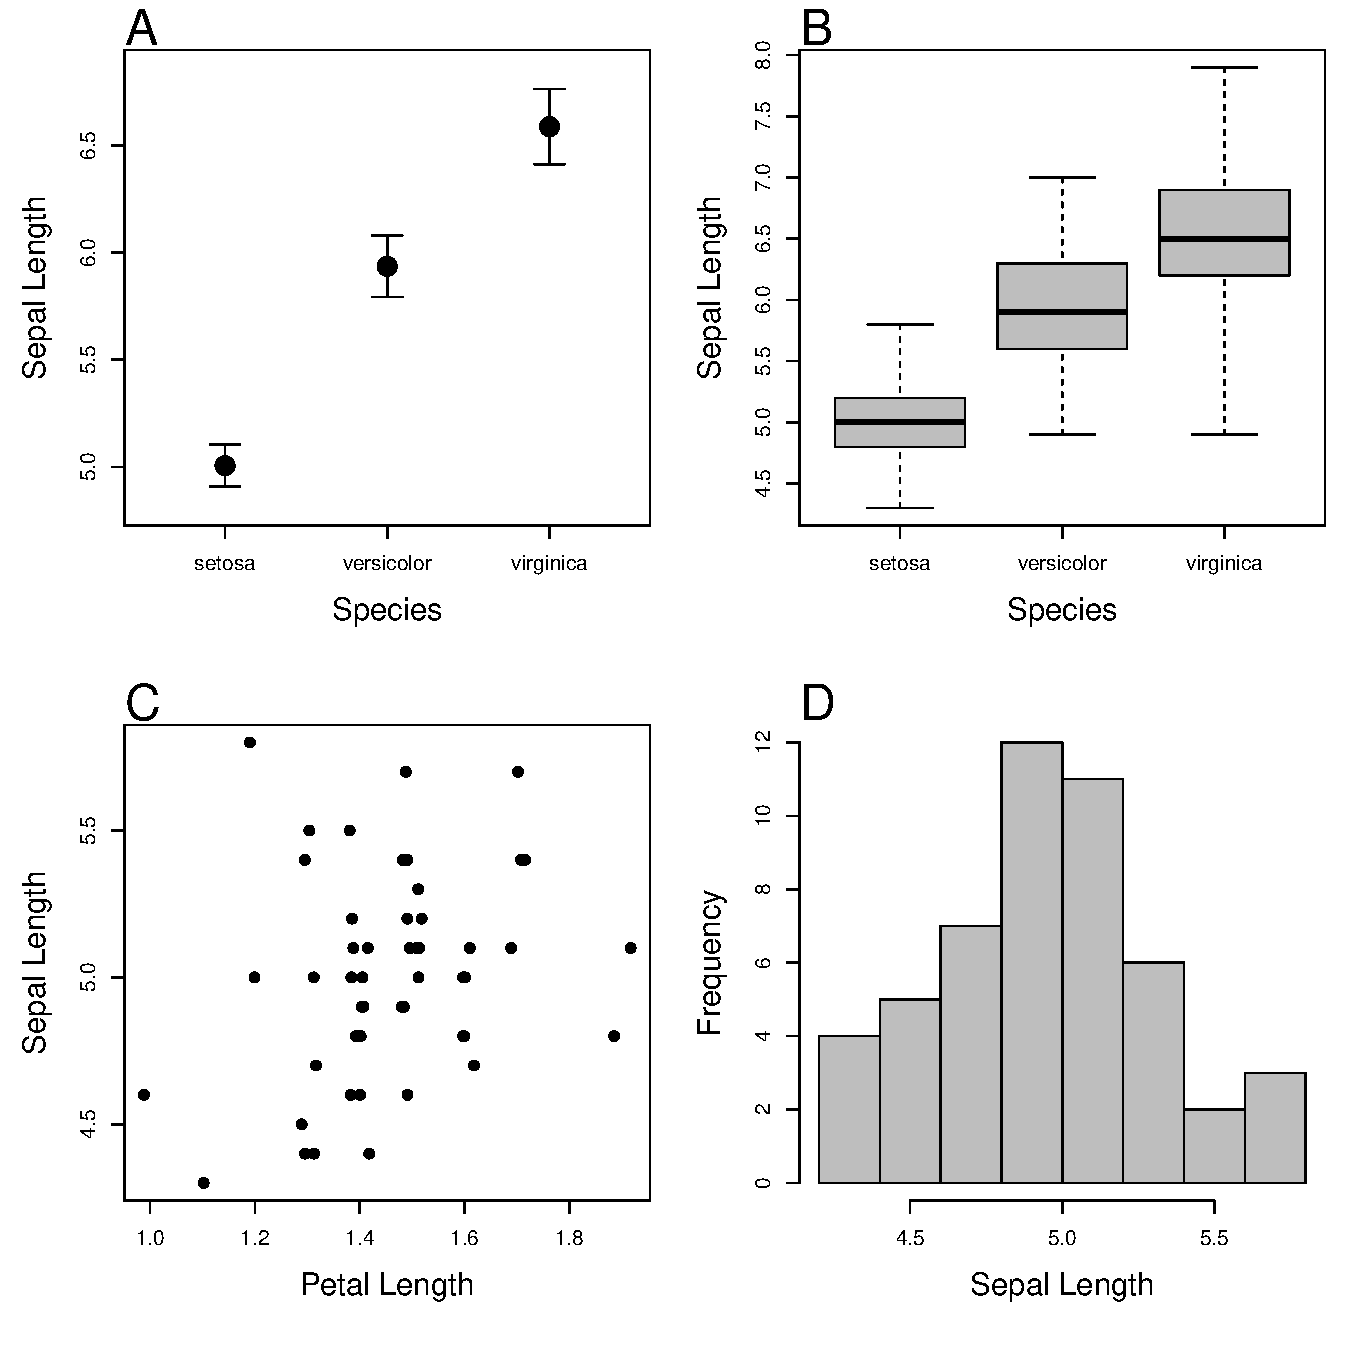
\includegraphics[width=0.9\textwidth]{fig_plot_type.pdf} 
 \caption{Four plot types that metaDigitise is designed to extract data from: A) mean and error plot, B) box plot, C) scatter plot and D) histogram. Data is taken from the iris dataset in R. A and B are plotted with the whole dataset, C and D are just the data for the species setosa.}
\label{fig:plot_type}
\end{figure}

\section*{Directory Structure and Reproducibility}

The `metaDigitise` package is quite flexible. There is one main function in the package, metaDigitise, which interactively takes the user through the process of extracting figures from graphs. `metaDigitise` can work on a directory with figures (currently .png, .jpg, .tiff, .pdf images can be used) from many different papers and that are of different types (see below). However, users can get creative in how they set up the directories of figures to facilitate extraction. For example, one might have 3–4 figures from a single paper that need extracting and the user may want to focus on a single paper at a time while the information about a paper is on hand. This could be done by simply setting up a file structure as follows and then using `metaDigitise` with path names (i.e., directory) for each papers folder:

\begin{lstlisting}
	* Main project directory
		+ Paper1_P1
			+ Figure1.png
			+ Figure2.png
			+ Figure3.png
		+ Paper2_P2
			+ Figure1.png
			+ Figure2.png
			+ Figure3.png
\end{lstlisting}

An alternative directory structure (and probably the most flexible) would be to simply have a set of different figures with an informative and relevant naming scheme to make it easy to identify the paper and figure the data come from. This cuts out the need to change directories constantly. For example the directory structure could look like:

\begin{lstlisting}
	* Main project directory
		+ FiguresToExtract
			+ P1_Figure1_trait1.png
			+ P1_Figure2_trait2.png
			+ P1_Figure3_trait3.png
			+ P2_Figure1_trait1.png
			+ P2_Figure2_trait2.png
			+ P2_Figure3_trait3.png
\end{lstlisting}

The above directory structure is probably the easiest in combination with a clear and unambiguous naming scheme for each figure. Even if only figures from a single paper are digitised, one paper at a time, an overall figure directory will work perfectly because `metaDigitise` will only cycle through incomplete figures, so figures can be added at anytime. 

Nonetheless, how users set up their directory is really up to them. However, it is important for users to think carefully about reproducibility at this stage. Would they like to share the entire project folder with colleagues? or would they prefer to simply share the image folder? The answers to these questions are important because relative path names are stored in `metaDigitise` objects, meaning that the directory structure (currently at least) needs to be the same for colleagues to re-load previously digitised objects. Therefore, the working directory needs to be set to either the "main project directory" or the "FiguresToExtract" directory and relative path names (e.g., users should specify dir = "./FiguresToExtract/" if setting the working directory to "Main project directory") used as opposed to absolute paths. This facilitates reproducibility should colleagues want to see the digitisations or integrate previously digitised figures with newly digitised figures. All users need to achieve this is to provide others with is the project or image folder.

\section*{High-throughput Digitisation of Figure(s) within a Directory}
metaDigitise was created with the idea that the user would likely have multiple images to extract from. It therefore operates in the same way whether the user has one or multiple images. It assumes that the user has put all the figures needed for extraction in one parent directory (see above). Users can extract single figures (if this is all they have) using the `metaDigitise` function with a path name to the directory with the file. However, often many figures need extracting from a single paper or set of papers. `metaDigitise` will also handle these situations seamlessly by simply cycling through all figures within a directory. This is useful because it expedites digitising figures by preventing users from having to constantly change directories and / or open new images. It operates by recognizing all the figures in a folder and bringing up each figure automatically allowing the user to click and enter relevant information about a figure as they go. All this information is then stored in a data frame or list at the end of the process, saving quite a bit of time. Users can stop mid-way through a folder by simply exiting after the last plot they have digitised. The data from completed figures will automatically be written to a special `caldat/` folder that is created when first executing the metaDigitise function. Digitised data along with metadata for figures are stored in caldat/ for later use and editing (see below).

In order to correctly extract data from figures metaDigitise always requires the user to calibrate the axes in the figure. To do this, the user is required to click on two known points on the axis in question, and then enter the value of those points in the figure (Figure \ref{fig:calibrate}). Using this information, metaDigitise then calculates the value of any clicked points in terms of the figure axes. In the case of mean and error plots and box plots, it calibrates only the y axis (assuming the x axis is redundant). For scatter plots and histograms both axes are calibrated.

\begin{figure}[!h] 
%\onehalfspacing
 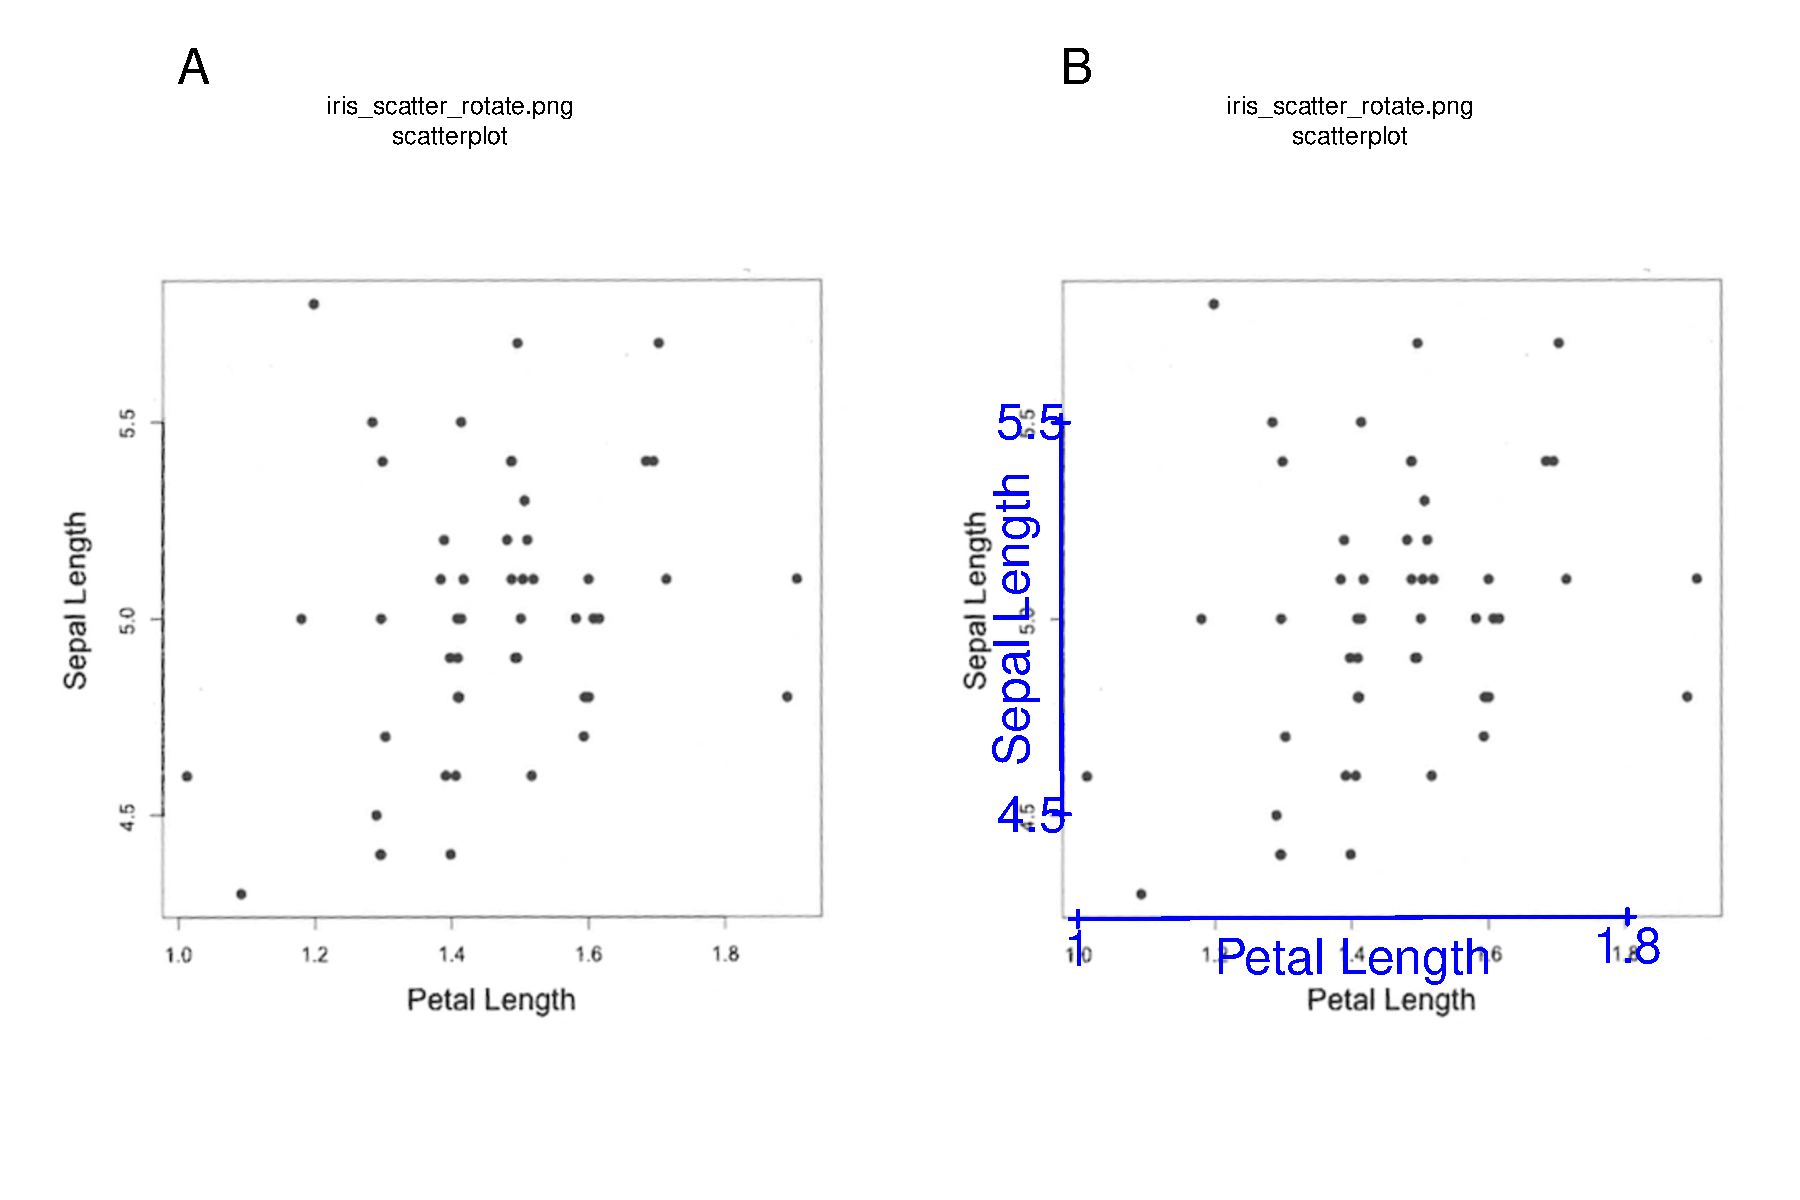
\includegraphics[width=0.9\textwidth]{fig_calibrate.pdf} 
 \caption{Axis calibration. The user defines two points on each axis and labels them according to the values shown in the figure.}
\label{fig:calibrate}
\end{figure}

A particularly powerful and flexible aspect of metaDigitise is its ability to recognize figures that are not already completed and only bring up those figures that have not been digitised in subsequent calls of the function. This means that new figures can be added at any time as the project develops and previously digitised figures are simply ignore during processing, but their data re-integrated within the final output after new files are completed. 

From all plot types, metaDigitise summarises the data from a figure or set of figures as a mean, standard deviation and sample size, for each identified group within the plot (should multiple groups exist). These are the summary statistics needed to create many of the relevant effect sizes and sampling error for a meta-analysis. In the case of scatter plots, metaDigitise also returns the correlation coefficient between the points within each identified group. 

\subsection{Diverse Plot Types}
metaDigitise recognises four main types of plot; Mean and error plots, box plots, scatter plots and histograms, shown in Figure \ref{fig:plot_type}. Each of these can be processed together and integrated into a single output. Alternatively, users can keep like figures together and process them separately.

%%% Equations for mean and sd
%% pooled stats: 
% \begin{align}
% \mu _{X}&={\frac {\sum _{i}{N_{X_{i}}\mu _{X_{i}}}}{\sum _{i}{N_{X_{i}}}}}
% \\
% \sigma _{X}&={\sqrt {{\frac {1}{\sum _{i}{N_{X_{i}}-1}}}\left(\sum _{i}{\left[(N_{X_{i}}-1)\sigma _{X_{i}}^{2}+N_{X_{i}}\mu _{X_{i}}^{2}\right]}-\left[\sum _{i}{N_{X_{i}}}\right]\mu _{X}^{2}\right)}}
% \end{align}


\begin{figure}[!h] 
%\onehalfspacing
 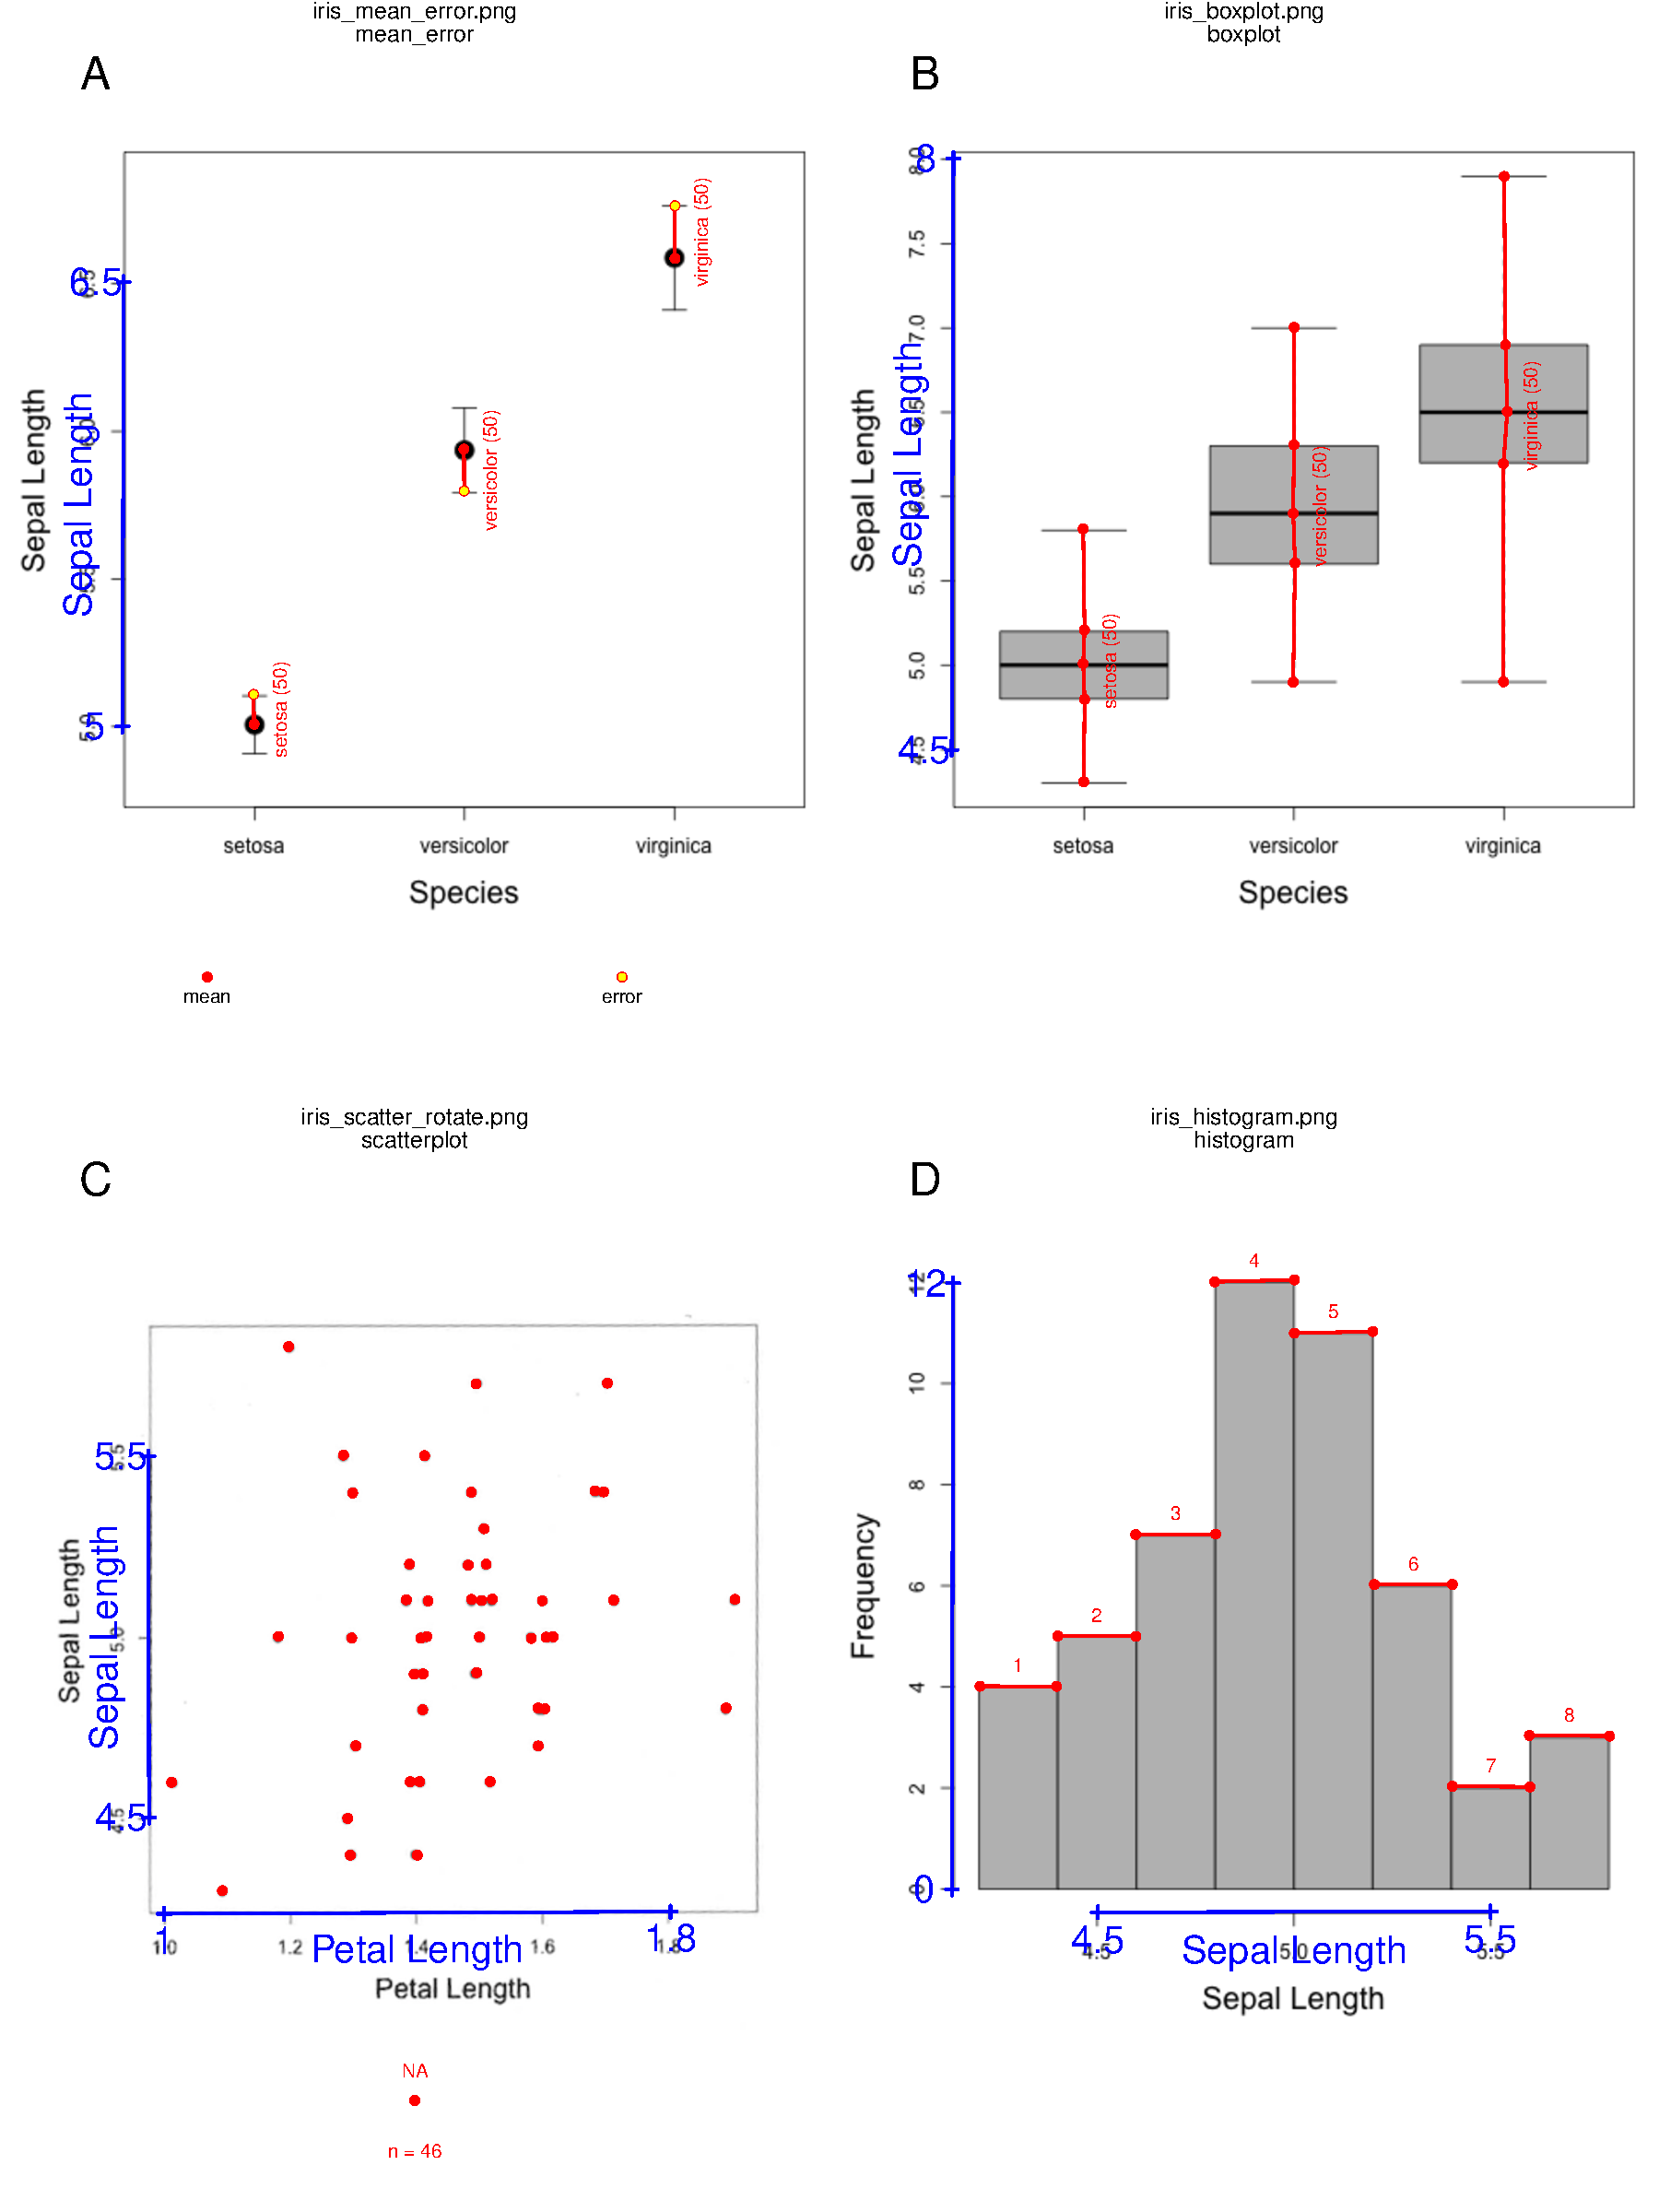
\includegraphics[width=0.9\textwidth]{fig_all_extract.pdf} 
 \caption{Demonstration of data extraction from different plot types}
\label{fig:all_extract}
\end{figure}

\subsubsection{Mean and error plots} 
metaDigitise prompts the user to enter groups names and allows the user to enter sample sizes, which are used in downstream processing. The user is then prompted to click on an error bar followed by the mean. Error bars above or below the mean can be clicked - sometimes one is clearer than the other. metaDigitise assumes that the error bars are symmetrical. Where the user has clicked the error is displayed in a different colour to the mean (Figure \ref{fig:all_extract}A). The user can subsequently add more groups or remove groups.

\subsubsection{Box plots}
 metaDigitise prompts the user to enter groups names and allows the user to enter sample sizes, which are used in downstream processing. The user is then prompted to click on the maximum, upper quartile, median, lower quartile and minimum. metaDigitise will check that the maximum is greater than the minimum, and return an warning if that is not the case. The user can subsequently add more groups or remove groups.

\subsubsection{Scatter plots}
 metaDigitise prompts the user to enter groups names and then to click on points. Points added by mistake can be deleted. The user can subsequently add groups, edit groups (add or remove points) or delete groups. Different groups are plotted in different colours and shapes, with a legend at the bottom of the figure (Figure \ref{fig:all_extract}C). The x and y coordinates are returned.

\subsubsection{Histograms}
metaDigitise prompts the user to enter groups names and then to click on the top corners of each bar. bars can subsequently be deleted. MetaDigitise then calculates the midpoint and the frequency for each bar. 

\subsection{Re-importing, Editing and Plotting Previously Digitised data}

A particularly useful feature of `metaDigitise` is its ability to re-import, edit and re-plot previously digitised figures. Running metaDigitise brings up a series of prompts for the user using a main menu that provides access to a number of its features: 

\begin{verbatim}
	Do you want to...
1: Process new images
2: Import existing data
3: Edit existing data
Selection: 
\end{verbatim}

The user simply enters in the numeric value that corresponds to what they would like to do. Choosing "Process new images" will permit users to digitise new figures, integrating previously completed digitisations along with newly digitised data together at the end of the session, or when the user decides to quit. If the user chooses "Import existing data", they have the option of either 1) importing all data or 2) importing a particular figure that has been digitised. If 2, then a list of files are provided to the user that they can select. 

Editing existing data allows users to easily re-plot or edit information or digitisations that have previously be done for any plot. This is accomplished by guiding the user through a new set of options:

\begin{verbatim}
Choose how you want to edit files:
1: Cycle through images
2: Choose specific file to edit
3: Enter previously omitted sample sizes
Selection: 
\end{verbatim}

If the user is unsure about the name of the specific figure they need to edit or simply want to just check the digitisations of figures they can choose "Cycle through images", which will bring up each figure, one by one, overlaying the calibrations, group names (if they exist), sample sizes (if they were entered) and the selected points. Alternatively, choosing option 2, will bring up a list of the completed files in the folder and the specific file can be chosen, at which point it will be replotted. Either of these options will cycle through a number of questions asking the user what they would like to edit:

\begin{verbatim}
Edit rotation? If yes, then the whole extraction will be redone (y/n) n
Change plot type? If yes, then the whole extraction will be redone (y/n) n
Variable entered as: Sepal length
Rename Variables (y/n) n
Edit calibration? (y/n) n
Re-extract data (y/n) y
Change group identifier? (y/n) n
Add group, Delete group or Finish plot? a/d/f d
1: setosa
2: versicolor
3: viriginica
Selection: 2
Add group, Delete group or Finish plot? a/d/f a
\end{verbatim}

A whole host of information can be edited from the rotation, plot type, the variable name that was provided, the calibration and even the digitisation of groups. When editing the metaDigitise object is re-written to the caldat folder and the edits are immediately integrated into the existing object once complete. 

\section{Additional Features}

\subsection{Figure Rotation and Adjustment}
Figure may have been extracted from old publications, for example from scanned images, and so are not perfectly orientated on the image. This will make the calibration of the points in the figure from the image problematic. metaDigitise allows users to rotate the image. By clicking two points on the x-axis, metaDigitse calculates the angle needed to rotate the image so the x-axis is horizontal, and rotates it. (Figure \ref{fig:rotate}A,B)

\begin{figure}[!h] 
%\onehalfspacing
 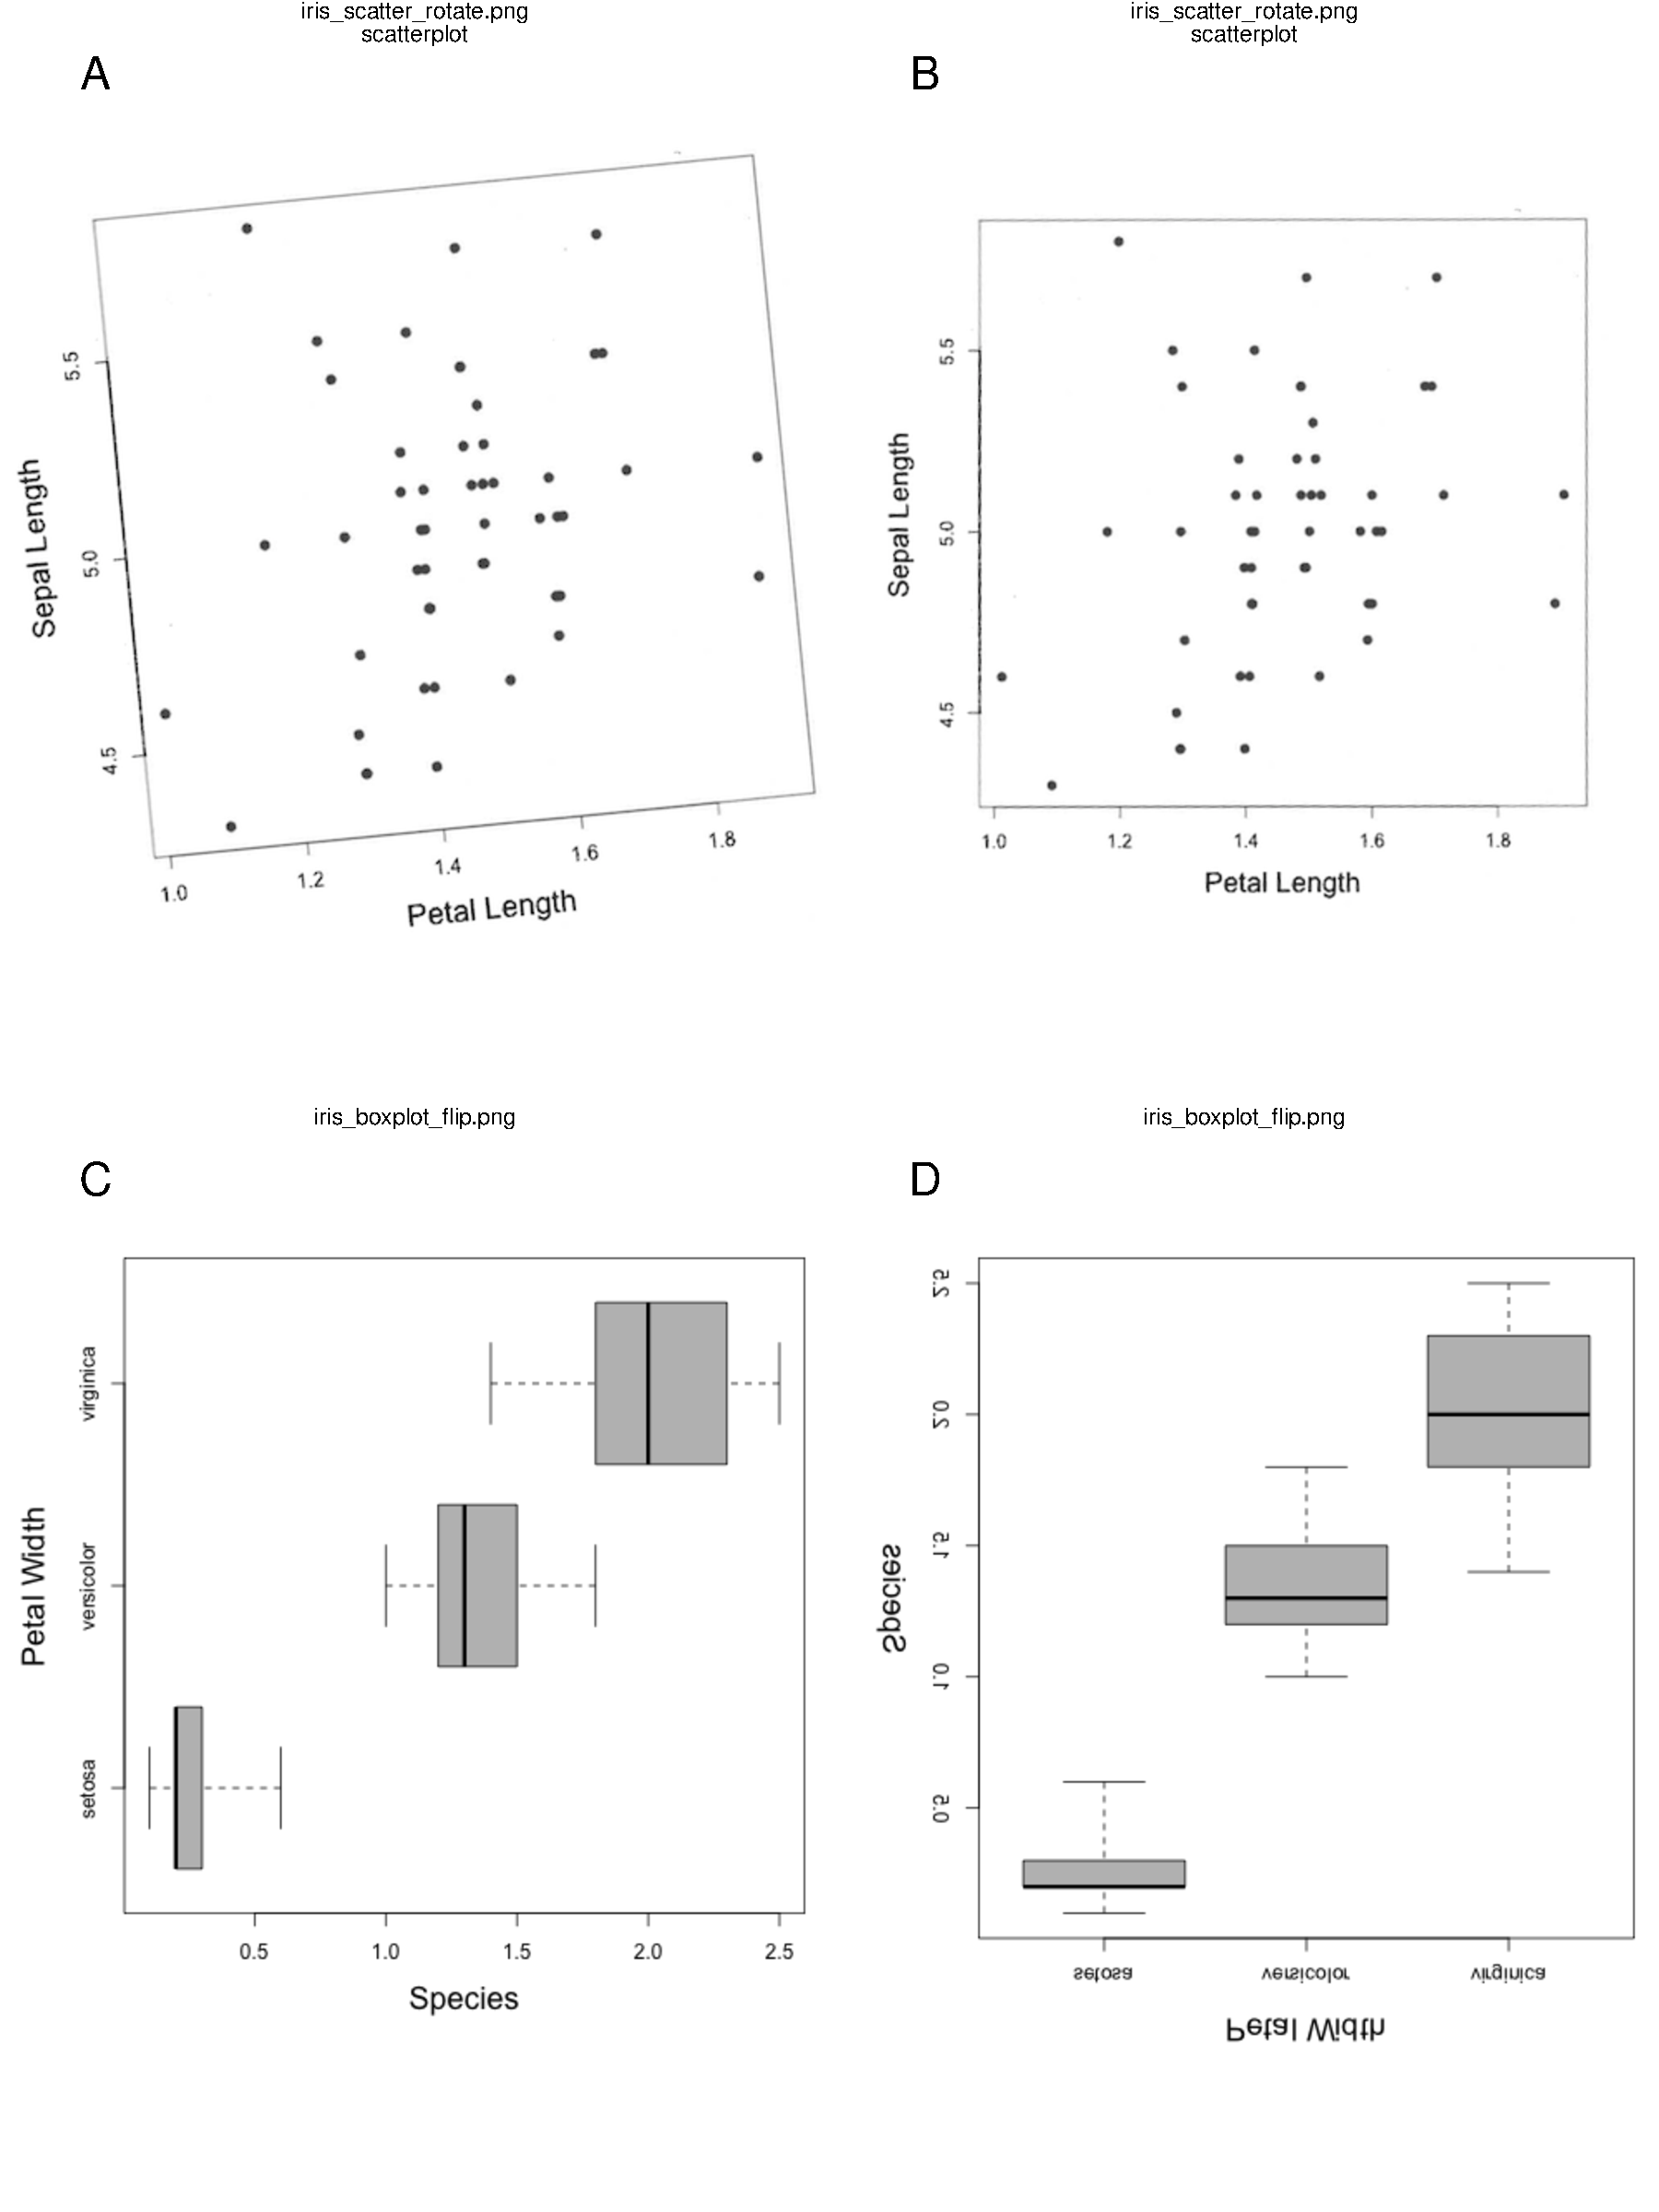
\includegraphics[width=0.9\textwidth]{fig_rotate.pdf} 
 \caption{Figure rotation. A) and B) show how non-aligned imaged can be realigned through user defined rotation. C) and D) show show figures can be re-orientated so as to aid data input.}
\label{fig:rotate}
\end{figure}

Furthermore, in some figures mean and error, boxplots or histograms may be presented with horizontal bars. metaDigitise assumes that the bars are vertical, but allows the user to flip the image so that the bars are vertical (Figure \ref{fig:rotate}C,D).

\subsection{Obtaining Raw Data}

While metaDigitise provides users with the summary statistics by default, for all plot types, in many cases the user may actually be interested in obtaining the raw digitised data from scatter plots. This is very easy to do my changing the default `summary` argument from TRUE to FALSE in the metaDigitise function. Instead of providing the user with summary statistics it will return a list containing four slots for each of the figure types (mean error, box plot, histogram and scatter plots). An example of a data object returned from digitising figures is as follows:

\begin{verbatim}
str(data)
List of 3
 $ mean_error :List of 1
  ..$ 002_Doe_2013_Fig1.png:'data.frame': 3 obs. of  5 variables:
  .. ..$ id      : Factor w/ 3 levels "setosa","versicolor",..: 1 2 3
  .. ..$ mean    : num [1:3] 5 5.93 6.59
  .. ..$ error   : num [1:3] 0.111 0.148 0.178
  .. ..$ n       : num [1:3] 50 50 50
  .. ..$ variable: chr [1:3] "Sepal length" "Sepal length" "Sepal length"
 $ hist       :List of 1
  ..$ 003_Doe_2013_Fig3.png:'data.frame': 8 obs. of  3 variables:
  .. ..$ midpoints: num [1:8] 4.3 4.5 4.7 4.9 5.1 ...
  .. ..$ frequency: num [1:8] 4 5 7 12 11 6 2 3
  .. ..$ variable : chr [1:8] "Sepal length" "Sepal length" "Sepal length" "Sepal length" ...
 $ scatterplot:List of 1
  ..$ 001_Anderson_1935_Fig1.png:'data.frame':  83 obs. of  8 variables:
  .. ..$ id        : Factor w/ 2 levels "setosa","versicolor": 1 1 1 1 1 1 1 1 1 1 ...
  .. ..$ x         : num [1:83] 2.3 2.9 3 3 3 ...
  .. ..$ y         : num [1:83] 4.5 4.4 4.41 4.3 4.8 ...
  .. ..$ group     : num [1:83] 1 1 1 1 1 1 1 1 1 1 ...
  .. ..$ col       : Factor w/ 2 levels "red","green": 1 1 1 1 1 1 1 1 1 1 ...
  .. ..$ pch       : num [1:83] 19 19 19 19 19 19 19 19 19 19 ...
  .. ..$ y_variable: chr [1:83] "Sepal length (mm)" "Sepal length (mm)" "Sepal length (mm)" "Sepal length (mm)" ...
  .. ..$ x_variable: chr [1:83] "Sepal width (mm)" "Sepal width (mm)" "Sepal width (mm)" "Sepal width (mm)" ...
\end{verbatim}

Here, the user can easily access the list of raw scatter plot data by simply extracting the scatter plot slot:

\begin{verbatim}
scatterplot <- data$scatterplot
\end{verbatim}

%check extraction
%Including addition of N later

\section{Example}
%% scatterplot from airquality data
We'll now turn to an example of how metaDigitise works using figures generated using the well known iris data set. Users can install metaDigitise from GitHub as follows:

\begin{verbatim}
	> install.packages("devtools")
	> devtools::install_github("daniel1noble/metaDigitise")
	> library(metaDigitise)
\end{verbatim}

Assume that we would like to extract summary statistics from studies measuring sepal length or width in iris species for a fictitious project. There are a few studies that only present these data in figures. As we read papers found from a systematic search we can add in figures with relevant data to a "figs\_to\_extract" folder as follows

\begin{lstlisting}
	*figs_to_extract
      + 001_Anderson_1935_Fig1.png
\end{lstlisting}

\begin{figure}[!h] 
%\onehalfspacing
 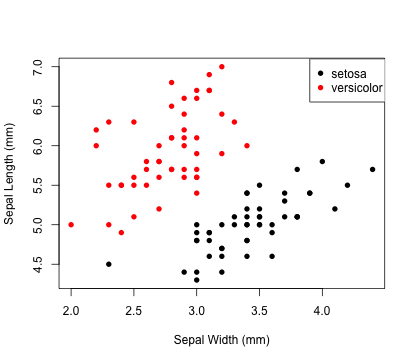
\includegraphics[width=0.9\textwidth]{001_Anderson_1935_Fig1.png} 
 \caption{Example scatterplot (001\_Anderson\_1935\_Fig1.png) of sepal length and width for two species of iris (setosa and versicolor)}
\label{fig:rotate}
\end{figure}

Here, the naming of the files placed in the folder will contain the paper number, first author and the figure number to keep data uniquely associated with figures. We can set our working directory to "figs\_to\_extract" and use metaDigitise to begin processing the image from the first paper

\begin{verbatim}
	> setwd("~/figs_to_extract")
	> digitised_data <- metaDigitise(".", summary = TRUE)
\end{verbatim}

As soon metaDigitise is executed, it will bring the user to the main menu (see "Re-importing, Editing and Plotting Previously Digitised data" above). When the user selects option one ("Process new images"), we are asked whether we have different types of plot(s) in the folder. This question is most relevant when there are lots of different figures in the folder because it will then ask us for the type of figure as they are cycled through.

\begin{lstlisting}
	Are all plot types the same? (diff/same)
\end{lstlisting}

metaDigitise then asks the user whether the figure needs to be rotated or flipped. This can be needed when box plots and mean and error plots are not orientated correctly. In some cases, older papers can give slightly off angled images which can be corrected by rotating. So, in this prompt the user has three options: `f` for "Flip", `r` for "rotate" or `c` for "continue. 

\begin{lstlisting}
	mean_error and boxplots should be vertically orientated
	       _ 
	       |  
	  I.E. o    NOT  |-o-|
	       |
	       _

	If they are not then chose flip to correct this.

	If figures are wonky, chose rotate.

	Otherwise chose continue

	Flip, rotate or continue f/r/c c
'\end{lstlisting}

After this, `metaDigistise` will ask the user to specify the plot type. Depending on the figure, the user can specify that it is a figure containing the mean and error (`m`), a box plot (`b`), a scatter plot (`s`) or a histogram (`h`). If the user has specified `diff` instead of `same` in response to the question about whether the plot types are the same or different, this question will pop up for each plot, but will only be asked once if plots are all the same. 

\begin{lstlisting}
	Please specify the plot_type as either: mean and error, box plot, scatter plot or histogram m/b/s/h:
\end{lstlisting}

After selecting the figure type a new set of prompts will come up that will ask the user first what the y and x-axis variables are. This is useful as users can keep track of the different variables across figures and papers. Here, the user can just add this information in to the R console. Once complete, details on how to calibrate the x and y-axis appear, so that the relevant statistics / data can be correctly calculated. When working with a plot of mean and standard errors, the x-axis is rather useless in terms of calibration so `metaDigitise` just asks the user to calibrate the y-axis. 

\begin{lstlisting}
What is the y variable? Sepal Length (mm)

What is the x variable? Sepal Width (mm)

On the Figure, click IN ORDER: 
      y1, y2 , x1, x2  


    Step 1 ----> Click on y1
  |
  |
  |
  |
  y1
  |_________________________
  ....

    Step 3 ----> Click on x1
  |
  |
  |
  |
  |
  |_____x1__________________

  ....
 \end{lstlisting}

The user can just follow the instructions on screen step-by-step (instructions above have been truncated by `...` to simplify), and in the order specified. Before moving on, the user is forced to check whether or not the calibration has been set up correctly. If `n` is chosen because something needs to be fixed then the user can re-calibrate.

\begin{lstlisting}
What is the value of y1 ?
4.5
What is the value of y2 ?
7
What is the value of x1 ?
2
What is the value of x2 ?
4

Re-calibrate? (y/n) 
\end{lstlisting}

Often, plots might contain multiple groups that the meta-analyst wants to extract from. `metaDigitise` handles this nicely by prompting the user to enter the group first, followed by the digitisation of this groups data. After digitising the first group, and having exited (i.e., hit `esc` from plot window), `mteaDigitise` will ask the user whether they would like to add another group. Users can continually add groups (`a`), or simply continue to the next plot (`c` - if another plot exists). The number of groups are not really limited and users can just keep adding in groups to accommodate the different numbers that may be presented across figures (although it can get complicated with too many).

\begin{lstlisting}
	Follow instructions below, to exit point adding or removing:

	 - Windows: right click on the plot area and choose 'Stop'!

	 - X11: hit any mouse button other than the left one.

	 - quartz/OS X: hit ESC

	Group identifier: setosa

	Click on points you want to add.
	If you want to remove a point, or are finished with a
	group, exit (see above), then follow prompts

	Add points, delete points or continue? a/d/c c

\end{lstlisting}

Once we are done digitising all the groups our plot will look something like this:

\begin{figure}[!h] 
%\onehalfspacing
 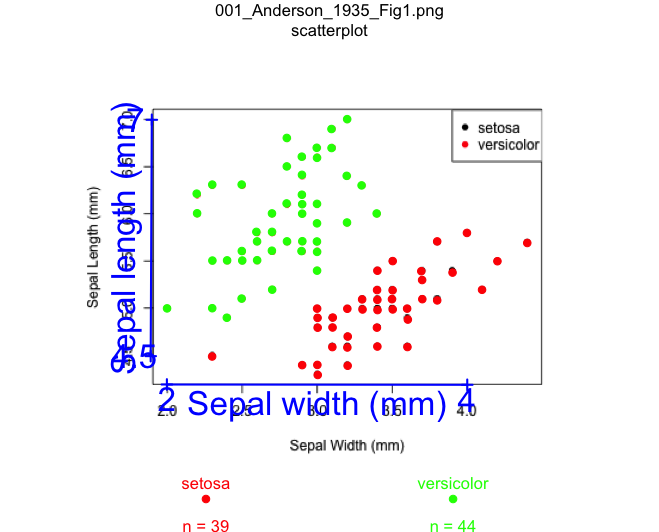
\includegraphics[width=0.9\textwidth]{001_Anderson_1935_Fig1_digitised.png} 
 \caption{Digitisation of sepal length and width for two species of iris (setosa and versicolor). Names of the variables and calibration (in blue) are plotted alongside the digitised points (green = versicolor; red = setosa). The sample sizes for each group are provided on the lower part of the plot. All figures are clearly labeled at the top to remind users of the filename and plot type. This reduces errors throughout the digitisation process.}
\label{fig:rotate}
\end{figure}

When completed metaDigitise will write the digitised data to the caldat directory, such that our new directory structure is as follows

\begin{lstlisting}
	*figs_to_extract
	  + caldat
	  	+ 001_Anderson_1935_Fig1
      + 001_Anderson_1935_Fig1.png
\end{lstlisting}

Users can access the metaDigitise object created (001\_Anderson\_1935\_Fig1) at any time using the metaDigitse function. In the R console, the summarised data for the digitised figure can be printed on screen or even written to a .csv file:

\begin{lstlisting}
data
                   filename   group_id         variable       mean      sd  n         r  plot_type
1 iris_scatter_multigrp.png     setosa  Sepal Width (mm) 3.420332 0.4034259 39 0.7524909 scatterplot
2 iris_scatter_multigrp.png     setosa Sepal Length (mm) 4.998267 0.3831294 39 0.7524909 scatterplot
3 iris_scatter_multigrp.png versicolor  Sepal Width (mm) 2.766857 0.3234723 44 0.5157938 scatterplot
4 iris_scatter_multigrp.png versicolor Sepal Length (mm) 5.936769 0.5292535 44 0.5157938 scatterplot
\end{lstlisting}

The mean for each of the two variables, along with the two species, are provided. Since this is a scatterplot, the user also gets the Person's correlation coefficient between sepal length and width for each species. These match reasonably well with the actual means of sepal length and width for each of the species in the full `iris` dataset:

\begin{lstlisting}
     Species meanSL meanSW
1     setosa  5.006  3.428
2 versicolor  5.936  2.770
\end{lstlisting}

One thing anyone with a familiarity with the iris dataset will notice is that the sample sizes for each of these species (which are n = 50 each) are quite a bit lower. This is an example of some of the challenges when extracting data from scatter plots, often data points will overlap with each other making it impossible (without having the real data) to know whether this is a problem. However, a meta-analyst will probably realise that the sample sizes here conflict with what is reported in the paper. Hence, metaDigitise also provides the user with  options to input the sample sizes directly (see Editing section above), even for scatter plots and histograms where, strictly speaking, this should not be necessary. Nonetheless, it is important to recognise the impact that overlapping points can have on summary statistics, particularly its effects on standard deviation (SD) and standard error (SE). Here, the mean point estimates are nearly bang on, but the SD's are slightly over-estimated:

\begin{lstlisting}
     Species    meanSL    meanSW
1     setosa 0.3524897 0.3790644
2 versicolor 0.5161711 0.3137983
\end{lstlisting}

\subsection{Adding new figures}

Users can add additional figures as new papers with relevant information are found. Each figure should be in its own file with unique naming, even if a single paper has multiple figures for extraction. For example, another paper on different populations (and one new species) of iris contained two additional figures where important data could be extracted. These figures can simply be named accordingly and added directly to the same extraction folder: 

\begin{lstlisting}
	*figs_to_extract
	  + caldat
	  	+ 001_Anderson_1935_Fig1
      + 001_Anderson_1935_Fig1.png
      + 002_Doe_2013_Fig1.png
      + 002_Doe_2013_Fig3.png
\end{lstlisting}

We have already processed one figure (001\_Anderson\_1935\_Fig1.png) and we can tell because it has digitised data (caldat/001\_Anderson\_1935\_Fig1), but now we have our two new figures that have not yet been digitised. This example will nicely demonstrate how users can easily pick up from where they left off and how all previous data gets re-integrated. It will also demonstrate how different plot types are handled. All we have to do to begin, is again, provide the directory where all the figures are located:

\begin{verbatim}
	> setwd("~/figs_to_extract")
	> digitised_data <- metaDigitise(".", summary = TRUE)
\end{verbatim}

The user gets the same set of prompts and simply chooses option one to digitise the new figures. This time, 001\_Anderson\_1935\_Fig1.png, is ignored and the new plots cycle on screen. First for 002\_Doe\_2013\_Fig1.png and then 002\_Doe\_2013\_Fig3.png. Since there are a few new figures, we answer the first question in the R console as "diff":

\begin{lstlisting}
	Are all plot types the same? (diff/same) diff


**** NEW PLOT ****

mean_error and boxplots should be vertically orientated
       _ 
       |  
  I.E. o    NOT  |-o-|
       |
       _

If they are not then chose flip to correct this.

If figures are wonky, chose rotate.

Otherwise chose continue

Flip, rotate or continue f/r/c c
Please specify the plot_type as either: mean and error, box plot, scatter plot or histogram m/b/s/h: m
\end{lstlisting}

Here, we specify the new plot type as `m` for 002\_Doe\_2013\_Fig1.png because we have a plot of the mean and error of sepal length for each of the three species. We're then prompted a bit differently from our scatter plot as the x-axis is not needed for calibration:

\begin{lstlisting}
What is the variable? Sepal length

On the Figure, click IN ORDER: 
      y1, y2  


    Step 1 ----> Click on y1
  |
  |
  |
  |
  y1
  |_________________________


    Step 2 ----> Click on y2
  |
  y2
  |
  |
  |
  |_________________________
  
What is the value of y1 ?
5
What is the value of y2 ?
6.5

Re-calibrate? (y/n) n

Enter sample sizes? y/n y

Group identifier: setosa

Group sample size: 50

Click on Error Bar, followed by the Mean

Add group, Delete group or Finish plot? a/d/f a
\end{lstlisting}
Again, metaDigitsie will simply guide the user through digitising each of these figures describing to them exactly what needs to be done. At any point if mistakes are made the user can choose relevant options to edit or correct things. This can continues for each plot so long as the user would like to continue after completing a single plot:

\begin{lstlisting}
Do you want continue: 1 plots out of 2 plots remaining (y/n) y
\end{lstlisting}

This continues until users have completed all non-digitised figures in the folder, at which point metaDigitise concatenates the new data with previously digitised data in the object:

\begin{lstlisting}
data
               filename        group_id         variable     mean        sd   n         r    plot_type
1 001_Anderson_1935_Fig1.png     setosa  Sepal Width (mm) 3.420332 0.4034259 39 0.7524909 scatterplot
2 001_Anderson_1935_Fig1.png     setosa Sepal Length (mm) 4.998267 0.3831294 39 0.7524909 scatterplot
3 001_Anderson_1935_Fig1.png versicolor  Sepal Width (mm) 2.766857 0.3234723 44 0.5157938 scatterplot
4 001_Anderson_1935_Fig1.png versicolor Sepal Length (mm) 5.936769 0.5292535 44 0.5157938 scatterplot
5      002_Doe_2013_Fig1.png     setosa      Sepal length 5.000336 0.7828656 50        NA  mean_error
6      002_Doe_2013_Fig1.png versicolor      Sepal length 5.931340 1.0466177 50        NA  mean_error
7      002_Doe_2013_Fig1.png viriginica      Sepal length 6.588705 1.2608173 50        NA  mean_error
8      003_Doe_2013_Fig3.png       <NA>      Sepal length 4.948472 0.3624212 50        NA  histogram
\end{lstlisting}

\section{Testing}
%% simulated data
%% x people doing y plots

\section{Conclusions and Future Enhancements}

mmetaDigitise is available through GitHub. WHile it is incredibly flexible already, our future plans include building in abilities to deal with log-transformed axes, including arguments for calculating standard deviations from 95\% confidence intervals and standard errors using the t-distribution to correct the t-value for small sample sizes (currently assumed t-values are 1.96 as is normal), dealing with asymmetric error bars and the possibility of zooming in plots such that greater accuracy can be achieved when digitising. We hope to also provide options for assessing inter-observer reliability in the future. 
\end{document}

